\chapter{Accounting for the vectorial nature of light propagation}
\label{ch:debye}



%Infinity corrected objectives enable a robust range of placements for the
%tube lens relative to the back aperture of the objective without noticeable
%loss in image quality. 

\section{Introduction}

The model for image formation outlined in \autoref{ch:hvm} provides a full
vectorial treatment of the propagation of the illuminating plane wave and
the resulting scattered fields up to the focal plane of the objective.
From there, it is assumed that the objective and tube lens simply magnify and
relay the intensity pattern in the focal plane to the camera plane.
This is a base assumption of traditional microscopy and is not unfounded; optics
manufacturers are economically incentivized to produce quality optics which
accurately image the specimen plane. However, these optics are optimized for
incoherent imaging of specimens in the focal plane.
How well does this venerable assumption hold for coherent imaging of out-of-plane
scatterers?

In this chapter, we will account for the propagation of the electric fields from
the specimen plane to the imaging plane. Our model includes the
refraction, reflection, and angular demagnification of the fields as they propagate
through the objective and tube lens before arriving at the camera plane.
We will attempt a full vectorial treatment throughout and will
validate any scalar wave approximations made along the way. In many ways our work
parallels and extends the work of Ovyrn and Izen\cite{izen00} and the work of
\c{C}apo\u{g}lu\cite{capoglu12} \emph{et al.} In particular, we adopt a similar
approach of the former and adopt the mathematical conventions and machinery of the latter.
Our work justifies the use of the scalar theory presented in \autoref{ch:hvm} and
probes the physical limits of HVM set by collecting, refocusing, and recording
the confluence of the incident beam and scattered wave.

\begin{figure}
  \centering
  \includegraphics[angle=90,origin=c,width=0.5\textwidth]{debye_wolf_schematic_rot}
  \caption{Diagram depicting the planes at which the fields will be evaluated.
    (a) The fields propagate through the focal plane (plane 1) of the objective.
    (b) The fields collected by the objective's entrance pupil (plane 2).
    (c) The fields are focused by the tube lens (plane 3) and arrive at the
    imaging plane (plane 4) of the camera.}
  \label{fig:debye_schematic}
\end{figure}

\section{Modeling the optical train}

With the exception of a coherent illumination source, our holographic microscope
can be reduced to the four essential components of a conventional microscope:
the sample, an objective, a tube lens, and a camera. In the previous chapter,
we described the scattering of a plane wave by a spherical scatterer up to
the focal plane of the objective. We will now evaluate the scattered field and
the plane wave at several interfaces as they propagate along the optical axis
to the camera plane. Figure \ref{fig:debye_schematic} illustrates the four planes
of interest. In the proceeding sections, we will perform the following calculations
for the scattered field:
\begin{enumerate}
\item Evaluate the electric field strength factor for the scattered field at
  the entrance pupil of the objective.
\item Account for the  $z_p$ displacement of the particle away from the focal
  plane of the objective.
\item Compute the electric field strength factor at the exit of the tube lens
  by accounting for the angular demagnification imposed by the objective.
\item Use the near-field-to-far-field transform to determine the scattered
  fields at the imaging plane of the camera.
\end{enumerate}
Owing to the linearity of our optical system, we may consider the incident field
and scattered field separately. We will derive the transformations for the
scattered field first and then summarize the resulting transformation for the
plane wave.

\subsection{Scattering to the entrance pupil}

In \autoref{ch:hvm} we computed the fields resulting from the scattering of
a plane wave from a homogeneous spherical inclusion in an otherwise
homogeneous medium. As depicted in Fig.~\ref{fig:debye_schematic}, we
propagate the radially expanding scattered fields through the focal plane (plane \num{1} in
Fig.~\ref{fig:debye_schematic}) and all the way to the objective's entrance pupil a distance
$z_p + f$ below the particle, where $f$ is the working distance of the objective.
Our objective  (Nikon Plan Apo, $\num{100}\times$, numerical aperture $\num{1.45}$,
oil immersion) was manufactured to have a working distance of $\SI{135}{\um}$.
At this distance, wavelength, and particle size, the scattered field is in the far-zone,
also known as the Fraunhofer zone, and the wave's $r$ dependence approximately
takes the following functional form:
\begin{equation*}
  \label{eq:strength_factor}
  \vec{E}(r, \theta, \phi) \approx \frac{\vec{E}(\theta, \phi)e^{ikr}}{r}
\end{equation*}
The term $\vec{E}(\theta, \phi)$ is known as the strength factor and it
has only $\theta$ and $\phi$ dependence. 

Casting the scattered field in terms of it's strength factor will simplify
several of the ensuing calculations. However, we have embedded an assumption
into our formalism: whenever the scattered field is not suitably in the far-field
regime, our formalism will break down. Ovyrn and Izen\cite{izen00} state
that the adoption of this approximation induces a maximum
$\SI{2}{\percent}$ error in their domain of interest. We conclude similarly in
\cite{app:lorenzmie_approx} for our domain of interest.

\section{ Displacement of the scattered field}

The electric field strength factor $\vec{E}(\theta, \phi)$ is independent
of distance; the fact that the scatterer is a distance $z_p$ away
from the focal plane will be lost in the near-field-to-far-field transform.
As described in  ``Introduction to Fourier Optics''\cite{goodman05},
the scatterer's displacement along the optical axis may be approximated by
a relative phase shift of the electric field strength factor
\begin{equation*}
  \label{eq:entrance_pupil}
    \vec{E}(\theta, \phi)|_{\text{scatter plane}} = \vec{E}(\theta, \phi)|_{\text{focal plane}} e^{-i\frac{2\pi}{\lambda}z\cos{\theta} }
  \end{equation*}
  
\footnote{In Goodman's text\cite{goodman05}, this would be a negative
  distance and yet in our geometry we have defined it to be a positive distance.
  Therefore we adopt Eq. 3-66 of Goodman with the alteration that  $z \rightarrow -z$.}

%The scattered field above gives an electric field strength factor that
%emanates from the origin of it's coordinate system. In the eyes of the
%collection step, this will mean that the scatterer is located at the origin
%of the focal plane. The scatterers we hope to investigate will be staged 
%some distance z above the focal plane such that the interefence patterns 
%culiminating in the camera plane will be maximally-information dense.

%Note, we will later adopt the direction cosines $(s_x, s_y)$ used in

\begin{figure}
  \centering
  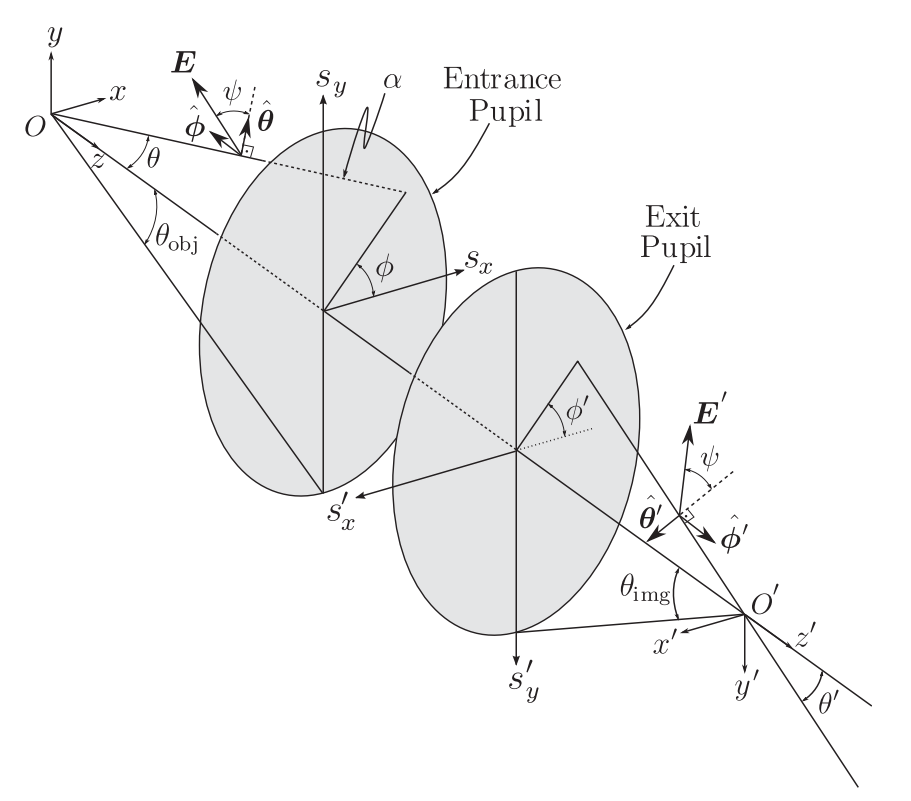
\includegraphics[angle=90,origin=c,width=0.5\textwidth]{debye_geom}
  \caption{The two spherical geometries necessary for our description.}
  \label{fig:debye_schematic}
\end{figure}

\section{Collection}
The scattered field experiences angular demagnification 
which imparts a scaling, polarization rotation, and lensing effect on all the rays passing
through the objective and tube lens. In total this effect can be accounted for by
a coordinate transformation governed by the abbe-sine condition and by scaling
each ray to obey the conservation of energy.

The abbe sine-condition is a necessary condition for sharp imaging:
\begin{equation*}
  M = \frac{n \sin \, \theta}{n^{\prime} \sin \, \theta^{\prime}}
  \label{eq:abbe_sine}
\end{equation*}
  and exquisitely obeyed my modern optics. Provided Eq.~\eqref{eq:abbe_sine}, a ray entering
  the objective at angle $\theta$ will exit the tube lens with angle $\theta^{\prime}$ as
  portrayed in Fig.~\ref{fig:debye_geom}. Additionally, the lens will impart a polarization
  rotation of $\SI{180}{\degree}$.

Here we will repeat the conservation of energy arguments present in section
1, but unlike the plane wave, we will find that the amplitude and 
polarization of the spherical wave is perturbed by the optical train in a 
$\theta$ dependent fashion. 

  \begin{equation*}
    \begin{split}
    \vec{E'}(\theta', \phi')\cdot\hat{\theta'} & = - M \sqrt{ \frac{n'\cos{\theta'}}{n\cos{\theta}}}\vec{E}(\theta, \phi)\cdot\hat{\theta}\\
    \vec{E'}(\theta', \phi')\cdot\hat{\phi'} & = - M \sqrt{ \frac{n'\cos{\theta'}}{n\cos{\theta}}}\vec{E}(\theta, \phi)\cdot\hat{\phi}
    \end{split}
  \end{equation*}

\section{Refocusing the fields to the camera plane}
The Debye-Wolf integral transforms the electric field strength factor at a lens
surface to the electric fields present in the focal plane of that lens.
\begin{equation*}
  \vec{E}_{img}(x', y') = \frac{i k'}{2 \pi} \iint_{\Omega_{img}} \vec{E'}_s(s'_x, s'_y) e^{-ik'(s'_xx'+s'_yy')}\frac{ds'_xds'_y}{\cos{\theta'}}
\end{equation*}

There are many things worth mentioning:
\begin{enumerate}
\item The Debye Wolf integral takes a field strength factor $\vec{E'}_s$,
  an integration domain $\Omega_{img}$ and the wavenumber $k'$ as it's inputs.
  From these inputs, the electric field in the (x'-y') plane is
  calculated. 
\item Heuristically, one should imagine that $\Omega_{img}$ dictates how far 
  away the plane (x'-y') will be (the distance scales with the size of 
  $\Omega_{img}$), that $k'$ gives the field strength factor the necessary 
  units to become an electric field and the electric field strength factor 
  contains most of the information detailing the interference pattern in the
  x'-y' plane ($k'$ has influence here as well).
\item This integral in many ways amounts to
  an inverse of Huygen's rule; a spherical wave is decomposed into a multitude 
  of plane waves whose phase relations and subsequent inteference produce
  the same effect as the original spherical wave.
\item The Debye-Wolf formalism easily accounts for any phase aberration 
  $\Phi(s'_x,s'_y)$ of the field as it passes through the optical train. To do so, the integrand
  of the Debye-Wolf integral is multiplied by a phase term $e^{ik'\Phi(s'_x,s'_y)}$.
\end{enumerate}

With the exception of the $k'$ in the phase term and the $\cos{\theta'}$ 
modifying the differential element, we should recognize the
Debye-Wolf integral as a fourier transform. We will discretize this
fourier transform subject to sampling and aliasing conditions described
in the appendix. I will simply summarize the reference's result and then
derive the minor cosmetic changes present in debyewolf.

\begin{equation*}
  \begin{split}
    \vec{E}_{img}( m \Delta_x, n \Delta_y) & \approx \frac{i k' \Delta s'_x \Delta s'_y}{2 \pi} e^{-i2\pi \left ( \frac{s'_{x_o}}{\Delta s'_x N_p} m + \frac{s'_{y_o}}{\Delta s'_yN_q} n \right ) } \vec{E}\left [ m, n \right ] \\
    \vec{E}\left [ m,n \right ] & = \sum_{p=0}^{N_p-1}\sum_{q=0}^{N_p-1}\vec{G'}\left [p,q\right ] e^{-i2\pi \left ( \frac{pm}{N_p}+\frac{qn}{N_q} \right ) } \\
    \vec{G'}(s'_x,s'_y) & \doteq \frac{\vec{E'}_s(s'_x,s'_y)}{\cos{\theta'}}e^{-ik'\Phi(s'_x,s'_y)}
  \end{split}
\end{equation*}

  

  Let's first reduce the prefactor in $\vec{E}_{img}$:
  \begin{eqnarray*}
    \frac{-ik'\Delta s'_x \Delta s'_y}{2 \pi} &=& -i\left ( \frac{k'}{2\pi} \right ) (2 \sin{\theta_{img}}/P)(2 \sin{\theta_{img}}/Q) \\
    &=& -i \left ( \frac{1}{\lambda'} \right ) \frac{4}{PQ} \left ( \sin{\theta_{img}} \right )^2 \hspace{.5 in} \text{By Equation 132. of Ref.}\\
    &=& -i \left ( \frac{1}{\lambda'} \right ) \frac{4}{PQ} \left ( \frac{\text{NA}}{Mn'} \right )^2 \\
    &=& -i \left ( \frac{4}{PQ} \right ) \left ( \frac{\text{NA}^2}{M^2\lambda n'} \right )
  \end{eqnarray*}

Now reduce the exponential in $\vec{E}_{img}$:
\begin{eqnarray*}
  i2\pi \left ( \frac{s'_{x_o}}{\Delta s'_x N_p} m + \frac{s'_{y_o}}{\Delta s'_yN_q} n \right )  &=& i2\pi \left ( \frac{-\sin{\theta_{img}} \left ( 1 - 1/P\right )}{2\sin{\theta_{img}}/P\cdot N_p} m + \frac{-\sin{\theta_{img}}\left ( 1-1/Q\right ) }{2\sin{\theta_{img}}/Q \cdot N_q} n \right ) \\
  &=& -i\pi \left ( \frac{P - 1}{N_p}m + \frac{Q - 1}{N_q} n \right ) 
\end{eqnarray*}
Therefore our expression for $\vec{E}_{img}$ is the following:

\begin{equation*}
  \vec{E}_{img} \approx -i \left ( \frac{4}{PQ} \right ) \left ( \frac{\text{NA}^2}{M^2\lambda n'} \right ) e^{-i\pi \left ( \frac{P - 1}{N_p}m + \frac{Q - 1}{N_q} n \right ) }\vec{E}\left [ m, n \right ]
\end{equation*}




Incident field:
\begin{enumerate}
\item[1.] Account for the phase displacement on the object side of the objective.
\item[2.] Account for the position independent lateral magnification.
\item[3.] Account for the phase displacement on the image side of the tube lens.
\end{enumerate}

We will assume the objective lens adequately obeys the abbe-sine condition.
In addition, we will trust that the objective obeys the conservation of energy
for all rays which enter it's pupil.
\begin{enumerate}
\item[1.] Compute the angular spectrum of the scattered field on a spherical surface
  in the far-field.
\item[2.] Apply the apodization caused by the entrance pupil of the objective.
\item[3.] Account for the direction dependent magnfication. This induces changes in
  amplitude, phase and direction (thus polarization).
\item[4.] Compute the electric fields present at the imaging plane from the angular spectrum in step 3.
\end{enumerate}

Finally the resulting image is computed with the poynting vector integrated over each pixel
\begin{equation*}
  I = \left | E_{inc} + E_{s} \right |^2.
\end{equation*}


\section{Propagating the incident field to the camera plane}
  The reference wave is assumed to be traveling coaxially through the optical
  train. It is collected by the objective, passed through ``infinity'' space
  and then rectified back to a plane wave. In the process, the field is flipped 
  (a $\pi$-shift in phase) but the polarization remains. 
  To maintain the conservation of energy, we should measure the flux of energy 
  a single, infinitesimal patch of the wave as it enters and exits the optical 
  train (see figure 1).

  \begin{eqnarray*}
    I_1 dA_1 &=& I_2 dA_2 \\
    \frac{n_1}{\eta_o} \left | \vec{E}_1 \right |^2 dA_1 &=& \frac{n_2}{\eta_o} \left | \vec{E}_2 \right |^2 dA_2\\
    \frac{n_1}{n_2} \left | \vec{E}_1 \right |^2 \frac{dA_1}{dA_2} &=& \left | \vec{E}_2 \right |^2 \\
    \frac{n_1}{n_2}  \frac{1}{M^2} \left | \vec{E}_1 \right |^2 &=& \left | \vec{E}_2 \right |^2 \hspace{.25 in}\text{magnification by M in -x,-y}\\
  \end{eqnarray*}

  By including the $\pi$-shift, we arrive at a final result for the plane wave:
  \begin{equation*}
    \vec{E}_2 = -\frac{1}{M}\sqrt{\frac{n_1}{n_2}} \vec{E}_1     
  \end{equation*}

  Until image formation, the following steps will exclusively refer to the 
  scattered field.


  
  In this work we have sought to produce an image in the camera plane from the
  fields present in the particle plane. To achieve such a transformation,
  we've treked through the optical train and accounted for various 
  effects including energy conservation, angular demagnification, polarization
  rotation, lensing effects and image formation. In doing so, we've
  implemented the Debye-Wolf formalism via a 2D fourier transform. To ensure that
  our sampling rate will not cause aliasing, we impose the following condition on
  the sampling number $P$ (the same argument applies to the sampling number $Q$):
  \begin{eqnarray*}
    \Delta s_x &<& \frac{2 \pi}{k W_x} \hspace{.5 in} \text{Eq 142 in Ref.}\\
    \frac{2 \sin{\theta_{img}}}{P} &<& \frac{\lambda}{W_x} \\
    \frac{2 \sin{\theta_{img}}W_x}{\lambda} &<& P \\
    \frac{2 \text{NA}\cdot W_x}{n\lambda} &<& P 
  \end{eqnarray*}
  
  The field $\vec{E}_{img}$ is discretized into a set of points 
  $\left ( \Delta_x, \Delta_y \right )$ in the camera plane. We desire that the
  spacing in the image approximates the real spacing between adjacent 
  pixels of our camera. As such, we seek to satisfy the relation 
  $\Delta_x = M\text{mpp}$. However, this is an integer equation which can only
  be approximately satisfied in general. Pursuing this approximation:
  \begin{eqnarray*}
    \Delta_x &\approx& \text{mpp}\cdot M \\
    \frac{2 \pi}{k' \Delta s_x' N_p} &\approx& \text{mpp}\cdot M \\
    \frac{\lambda'}{N_P} \frac{1}{\Delta s_x'} &\approx& \text{mpp}\cdot M \\
    \frac{\lambda'}{N_P} \frac{P}{2 \sin{\theta_{img}}} &\approx& \text{mpp}\cdot M \\
    \frac{\lambda'}{N_P} \frac{PMn'}{2\text{NA}} &\approx& \text{mpp}\cdot M \\
    \frac{\lambda}{N_P} \frac{P}{2\text{NA}} &\approx& \text{mpp} \\
    \frac{P\lambda}{2\text{NA}\cdot\text{mpp}} &\approx& N_p \\
    \frac{P\lambda}{2\text{NA}\cdot\text{mpp}} &\approx& P+\text{pad}_P \\
    \left ( \frac{\lambda}{2\text{NA}\cdot\text{mpp}} - 1 \right )P &\approx& \text{pad}_P \\    
  \end{eqnarray*}

  \begin{equation*}
    \begin{split}
      P > \frac{2 \text{NA}\cdot W_x}{n\lambda} \\
      \text{pad}_P  \approx  \left ( \frac{\lambda}{2\text{NA}\cdot\text{mpp}} - 1 \right )P
    \end{split}
  \end{equation*}


  
\section{Comparison to Scalar Diffraction Theory}


\begin{figure}
  \centering
  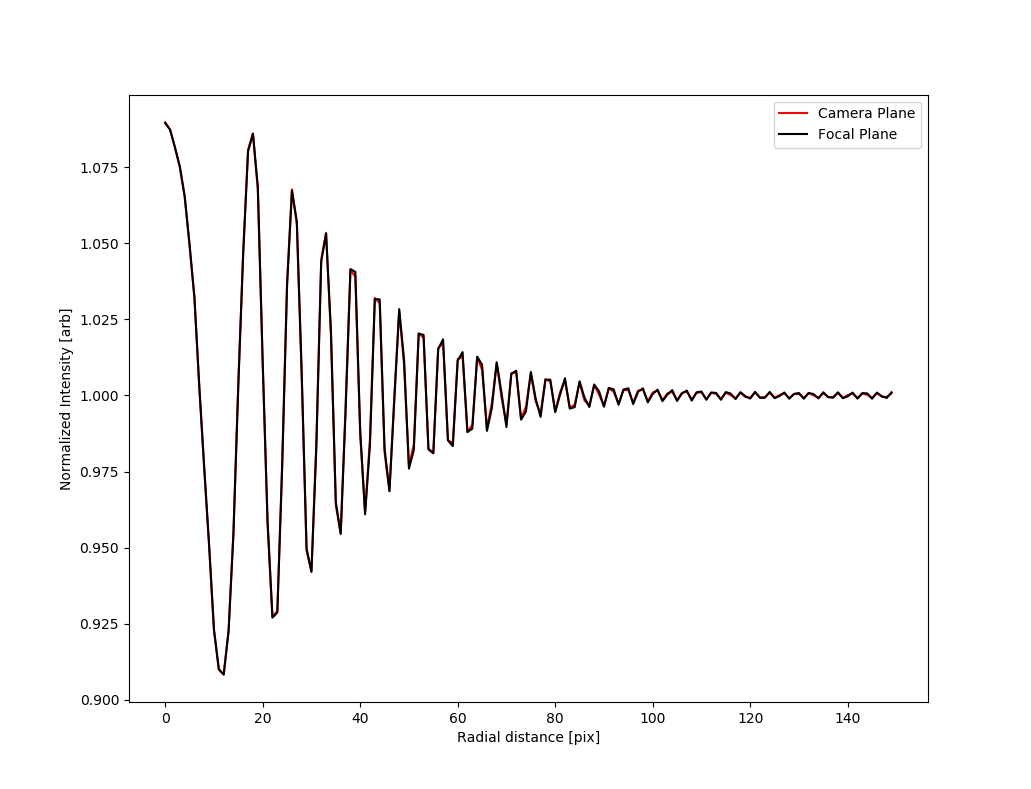
\includegraphics[width=\textwidth]{debye_difference_ps}
  \caption{Comparing the radial profiles of a holographic snapshot taken
    in the focal plane of the objective and the imaging plane of the camera.
    This particular holographic feature is produced by a $\SI{1.0}{\um}$
    diameter polystyrene particle $\SI{13.5}{\um}$ above the focal plane.}
  \label{fig:debye_difference_ps}
\end{figure}


\section{Discussion}

Not much to discuss yet.


